\documentclass[titlepage, 12pt]{article}

\usepackage{framed}
\usepackage{enumitem}
\usepackage{geometry}
\geometry{
  letterpaper,
  margin=1in,
}

\usepackage{graphicx}
\graphicspath{{./images/}}
\usepackage{float}
\usepackage{subcaption}

\title{SE 2XB3 Group 4 Report 3}
\author{
  Huang, Kehao \\
  400235182 \\
  \texttt{huangk53@mcmaster.ca} \\
  L01
  \and
  Jiao, Anhao \\
  400251837 \\
  \texttt{jiaoa3@mcmaster.ca} \\
  L01
  \and
  Ye, Xunzhou \\
  400268576 \\
  \texttt{yex33@mcmaster.ca} \\
  L01
}
\date{5 February 2021}

\begin{document}
\maketitle{}

\newpage{}

\section{Quicksort}

\subsection{In-Place Version}
\label{sec:in-place}

Our implementation has its natural in-place advantage over the given
implementation which uses auxiliary memory to store different partitions for
each recursion call. Specifically, our in-place implementation swaps elements in
the array and uses two parameter \texttt{low} and \texttt{high} to mark the
array partition on which a recursion call should work. The amount of memory used
for the whole sorting process is independent of the input size. In this case, it
is the length of the input array. On the other hand, the given non-in-place
implementation copies elements from the input array to fresh allocated auxiliary
arrays. Each auxiliary array is used as the new partition for the subsequent
recursion call. And the returned sorted array is a concatenation of two sorted
partitions and the pivot. Both the element copying action and list concatenation
are costly, in terms of both time and space complexity.

A test on the average runtime of both versions of quicksort is then carried out.
For \( n \) on the scale from \( 10^4 \) to \( 10^7 \), an array of \( n \)
random numbers is passed to both implementations. The runtime is plotted on a
semi-log graph as shown in Figure \ref{fig:ip-ax}. The experimental result did
not precisely match our prediction. From \( n = 10^4 \) to approximately \( n =
10^{5.5} \), the in-place version has a slight longer runtime than the
non-in-place version. Figure \ref{fig:ip-ax-zoomed} is a zoomed-in view of the
plot, which demonstrates the shorter runtime of the non-in-place version. As \(
n \) increases from \( 10^{5.5} \), the in-place quicksort gradually starts to
outperform the other. The disadvantage of using auxiliary arrays and deep
copying data around memory becomes obvious as \( n \) passes \( 10^6 \).

\begin{figure}[h]
  \centering
  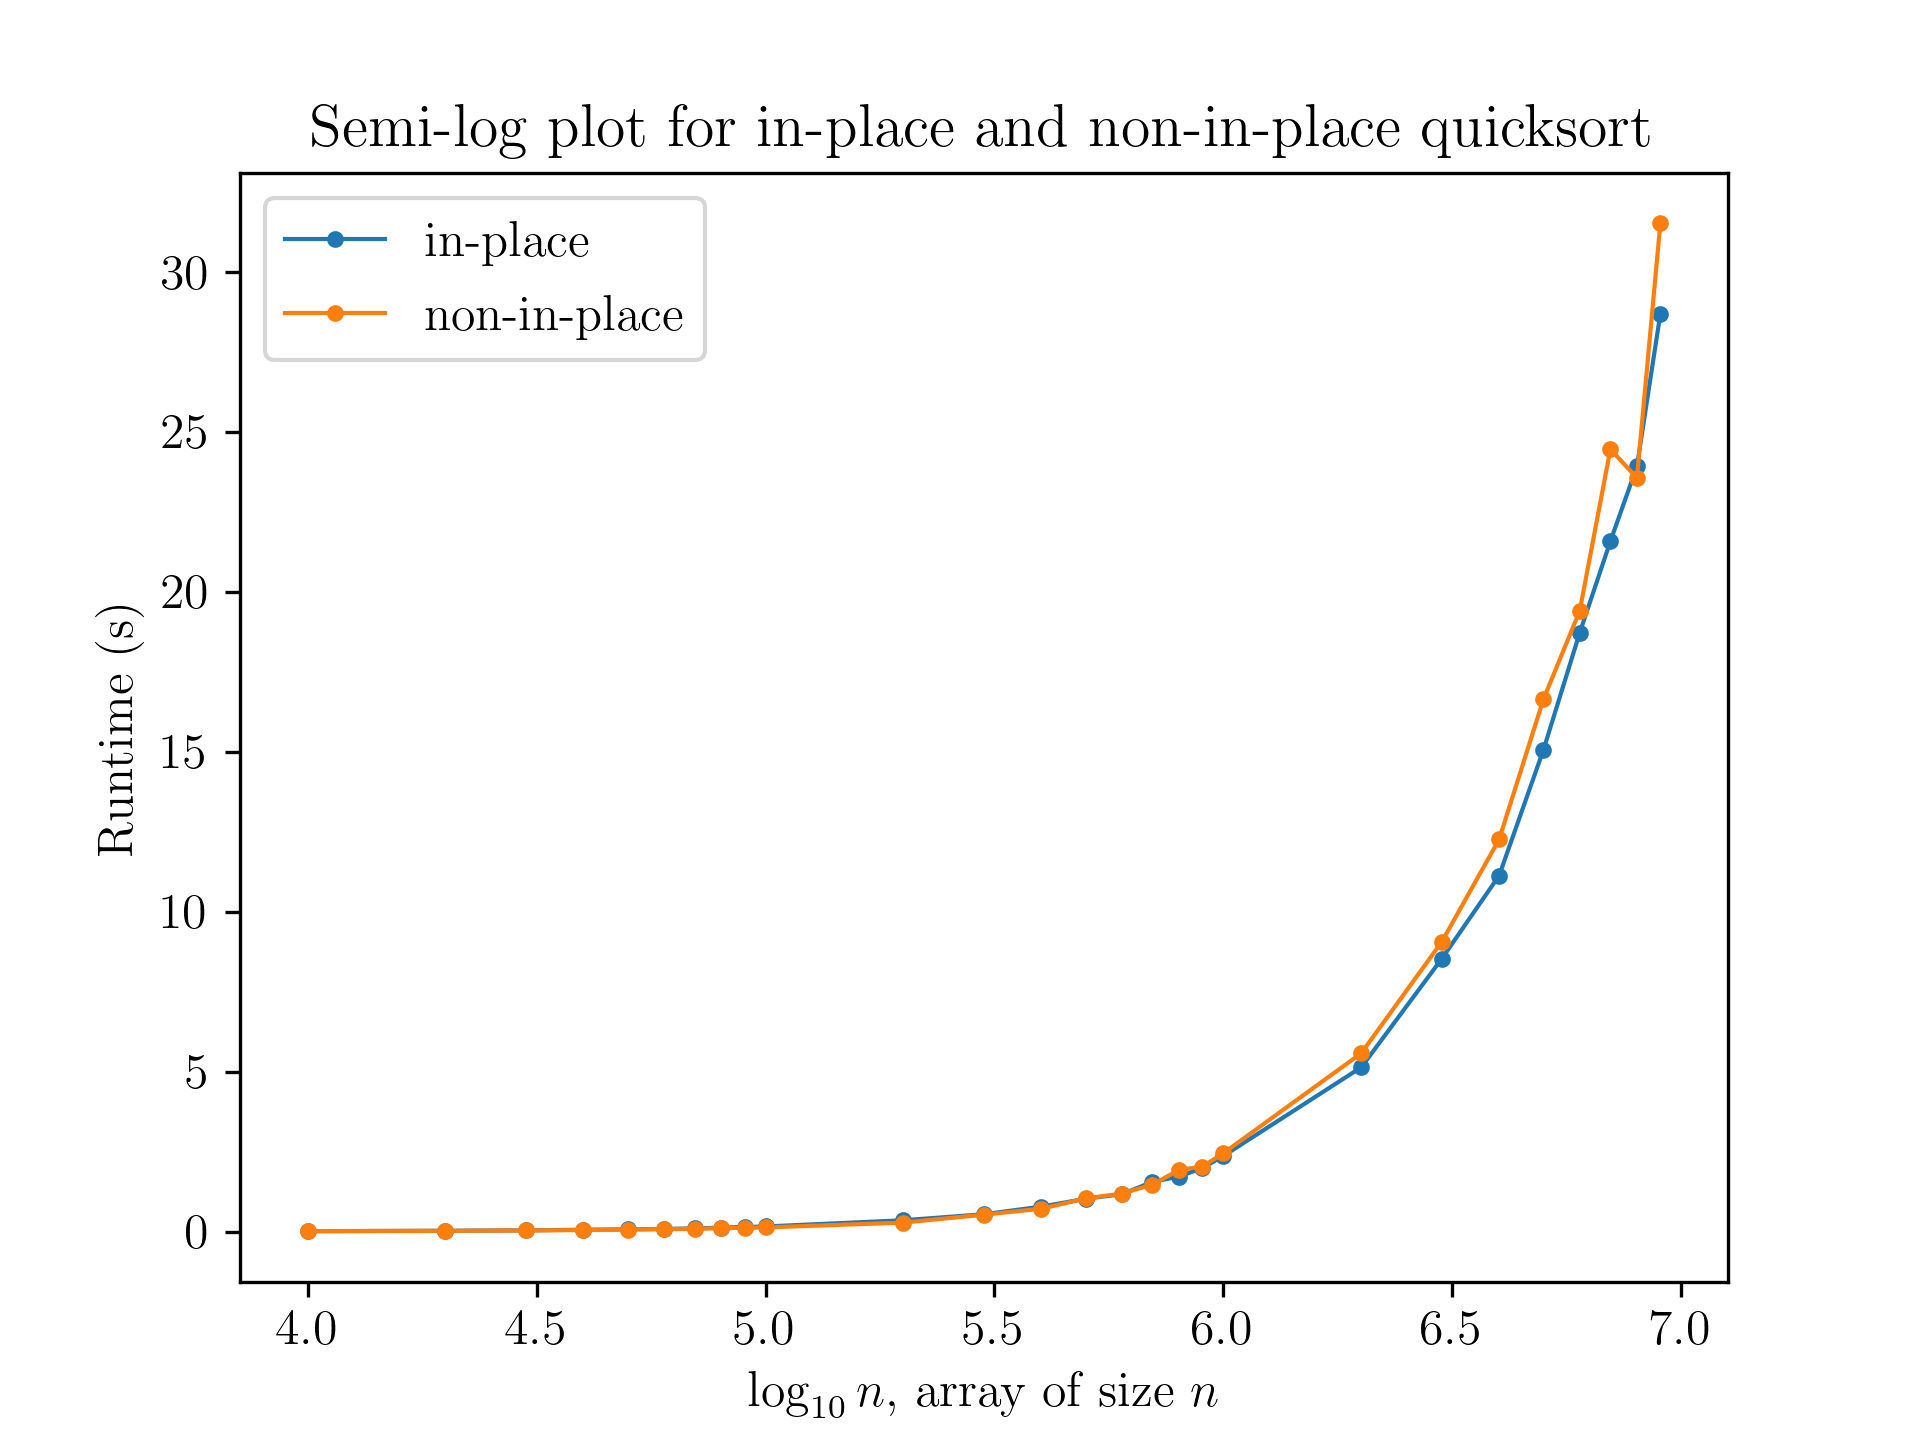
\includegraphics[width=0.8\textwidth]{ip-ax}
  \caption{In-place and non-in-place quicksort comparison}
  \label{fig:ip-ax}
\end{figure}
\begin{figure}[h]
  \centering
  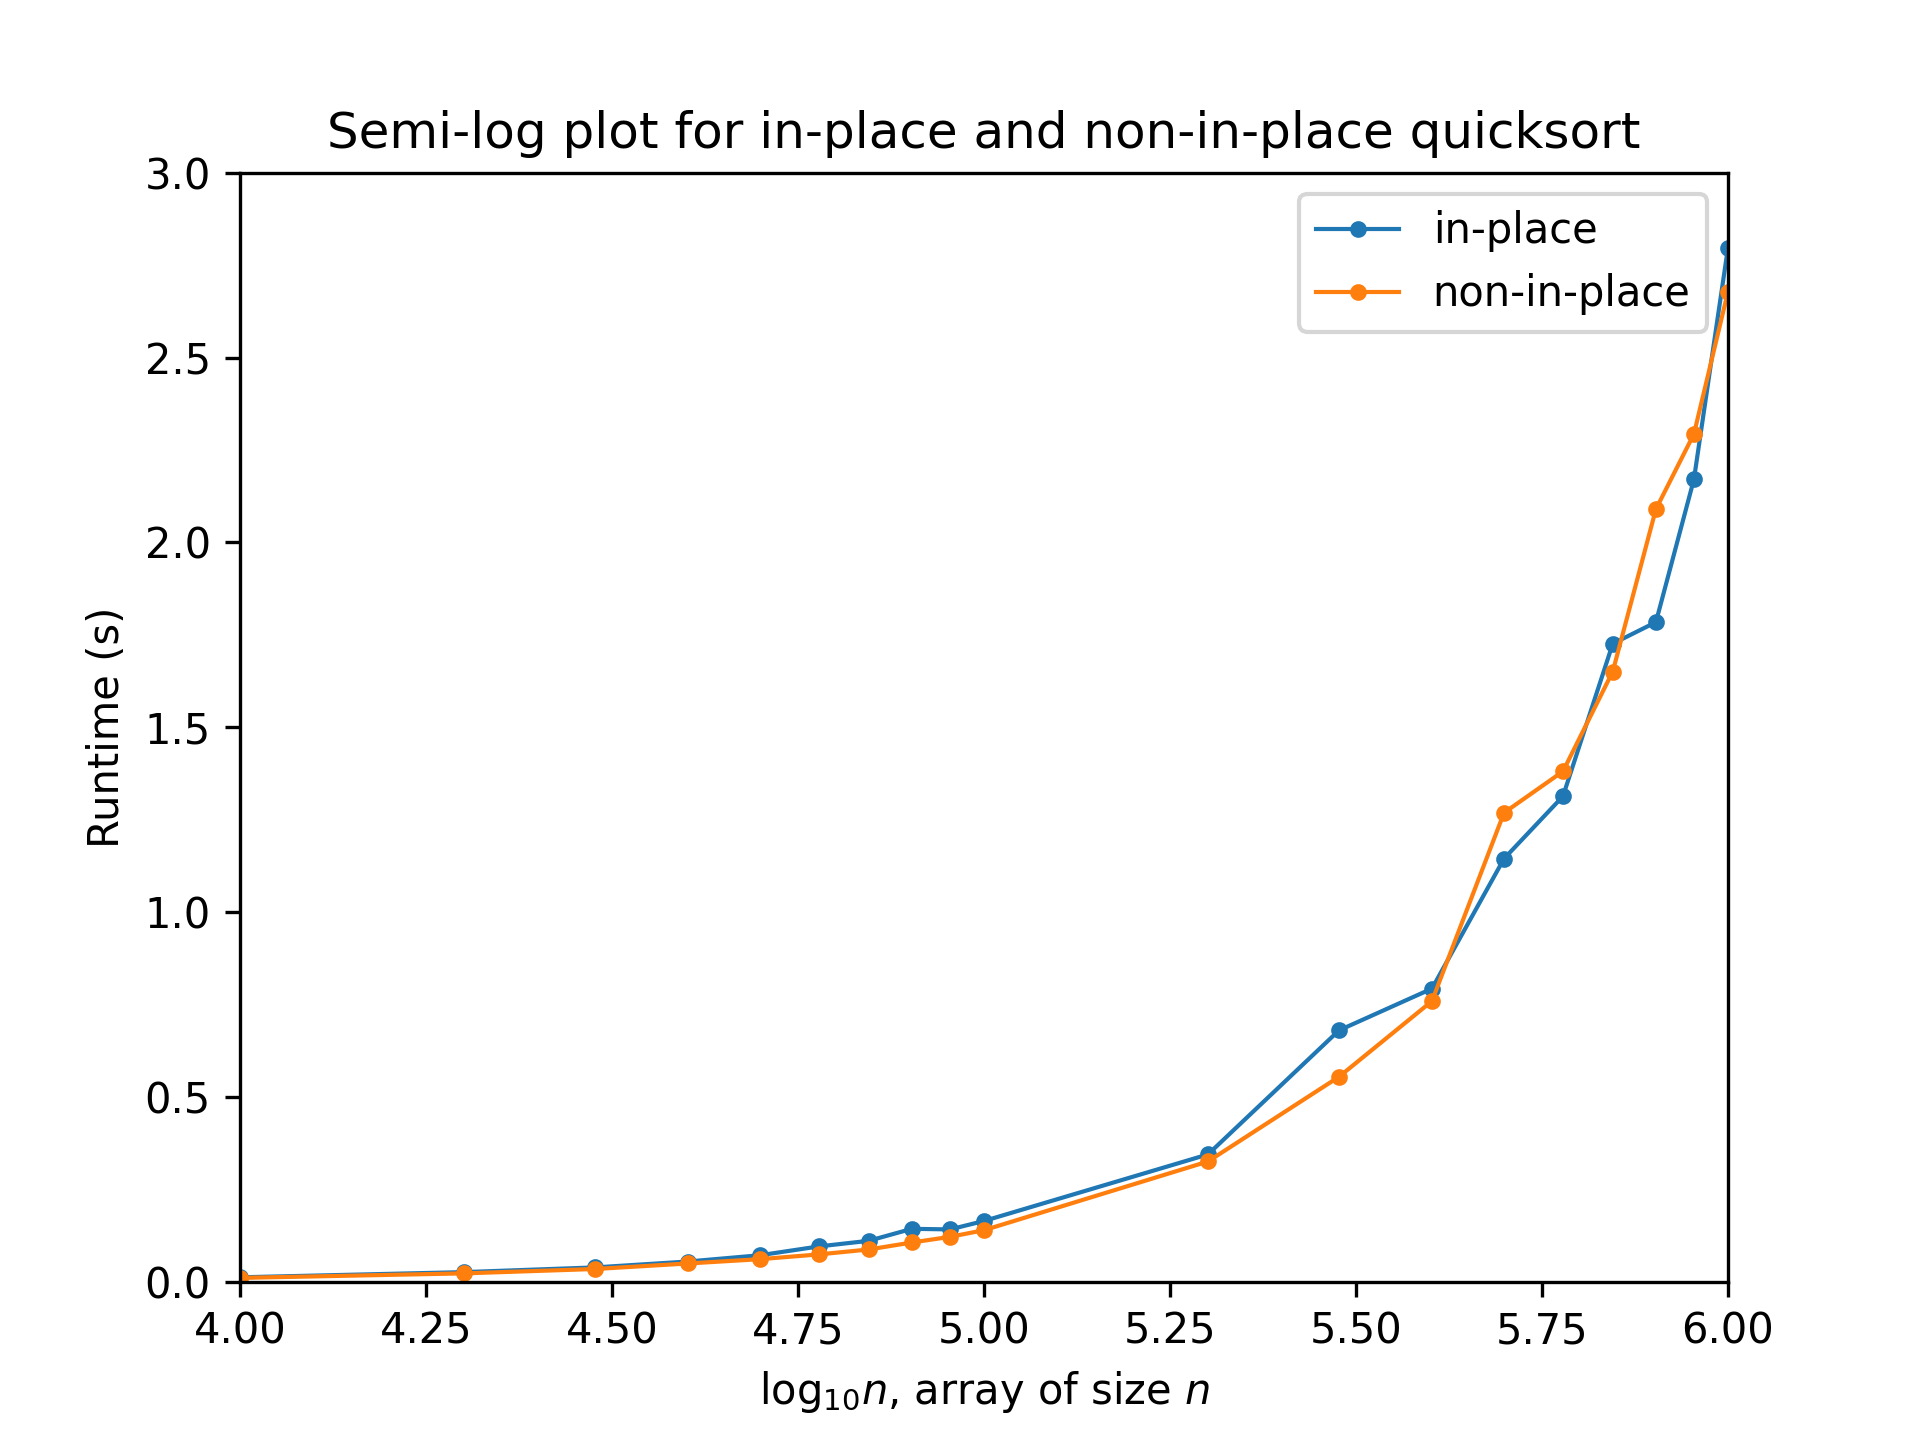
\includegraphics[width=0.8\textwidth]{ip-ax-zoomed} 
  \caption{Quicksort versions comparison on lower scale \( n \)}
  \label{fig:ip-ax-zoomed}
\end{figure}

To quantify the performance difference between the two versions, we used a
rather simple model. Either version of quicksort is known to have a complexity
of \( \mathcal{O}(n\lg{n}) \). We use \( c * n\lg{n} \) as an approximate model
of the imperial runtime. Thus we take the average of the differences of the \( c
\) constants of the two versions as the quantified performance difference. From
the same data set plotted above, for \( 10^4 \leq n < 10^7 \), the non-in-place
version is on average 4\% faster than the in-place version.

In conclusion, the non-in-place quicksort is slightly faster than the in-place
one in practice. However, the in-place version has an observable speed
improvement for an input size \( n > 10^6 \).

\subsection{Multi-Pivot}
\label{sec:multp}

Variants of quicksorts with different numbers of pivots were implemented and
tested against the traditional single-pivot quicksort. It is worth noting that
within the implementations of the quicksorts with two or more pivots, the
provided single-pivot quicksort is used to sort the chosen pivots and any input
array of length less than the number of pivots.

The performance of the quicksort variants was tested using arrays of length \(
10^4 \leq n < 10^7 \) (input size). As a result, the quad-pivot quicksort
outperformed the other sorting algorithms and was chosen as the recommended
quicksort. As shown in Figure \ref{fig:multp}, given an input size, the
quicksort finished faster as the number of pivots increased. The runtime
differences between variants widened as the input size increased. However, the
time advantage of the quad-pivot variant is only significant in the input range
\( n > 10^6 \). Figure \ref{fig:multp-zoomed} provide the zoomed-in views for \(
10^4 \leq n \leq 10^5 \) and \( 10^4 \leq n \leq 10^6 \). The performance of all
algorithms is rather unstable in these two ranges. There is no clear superior
out of the four tested variants. Therefore, the quad-pivot quicksort is
concluded to be the fastest solely based on its better performance on large
sized inputs.

\begin{figure}[h]
  \centering
  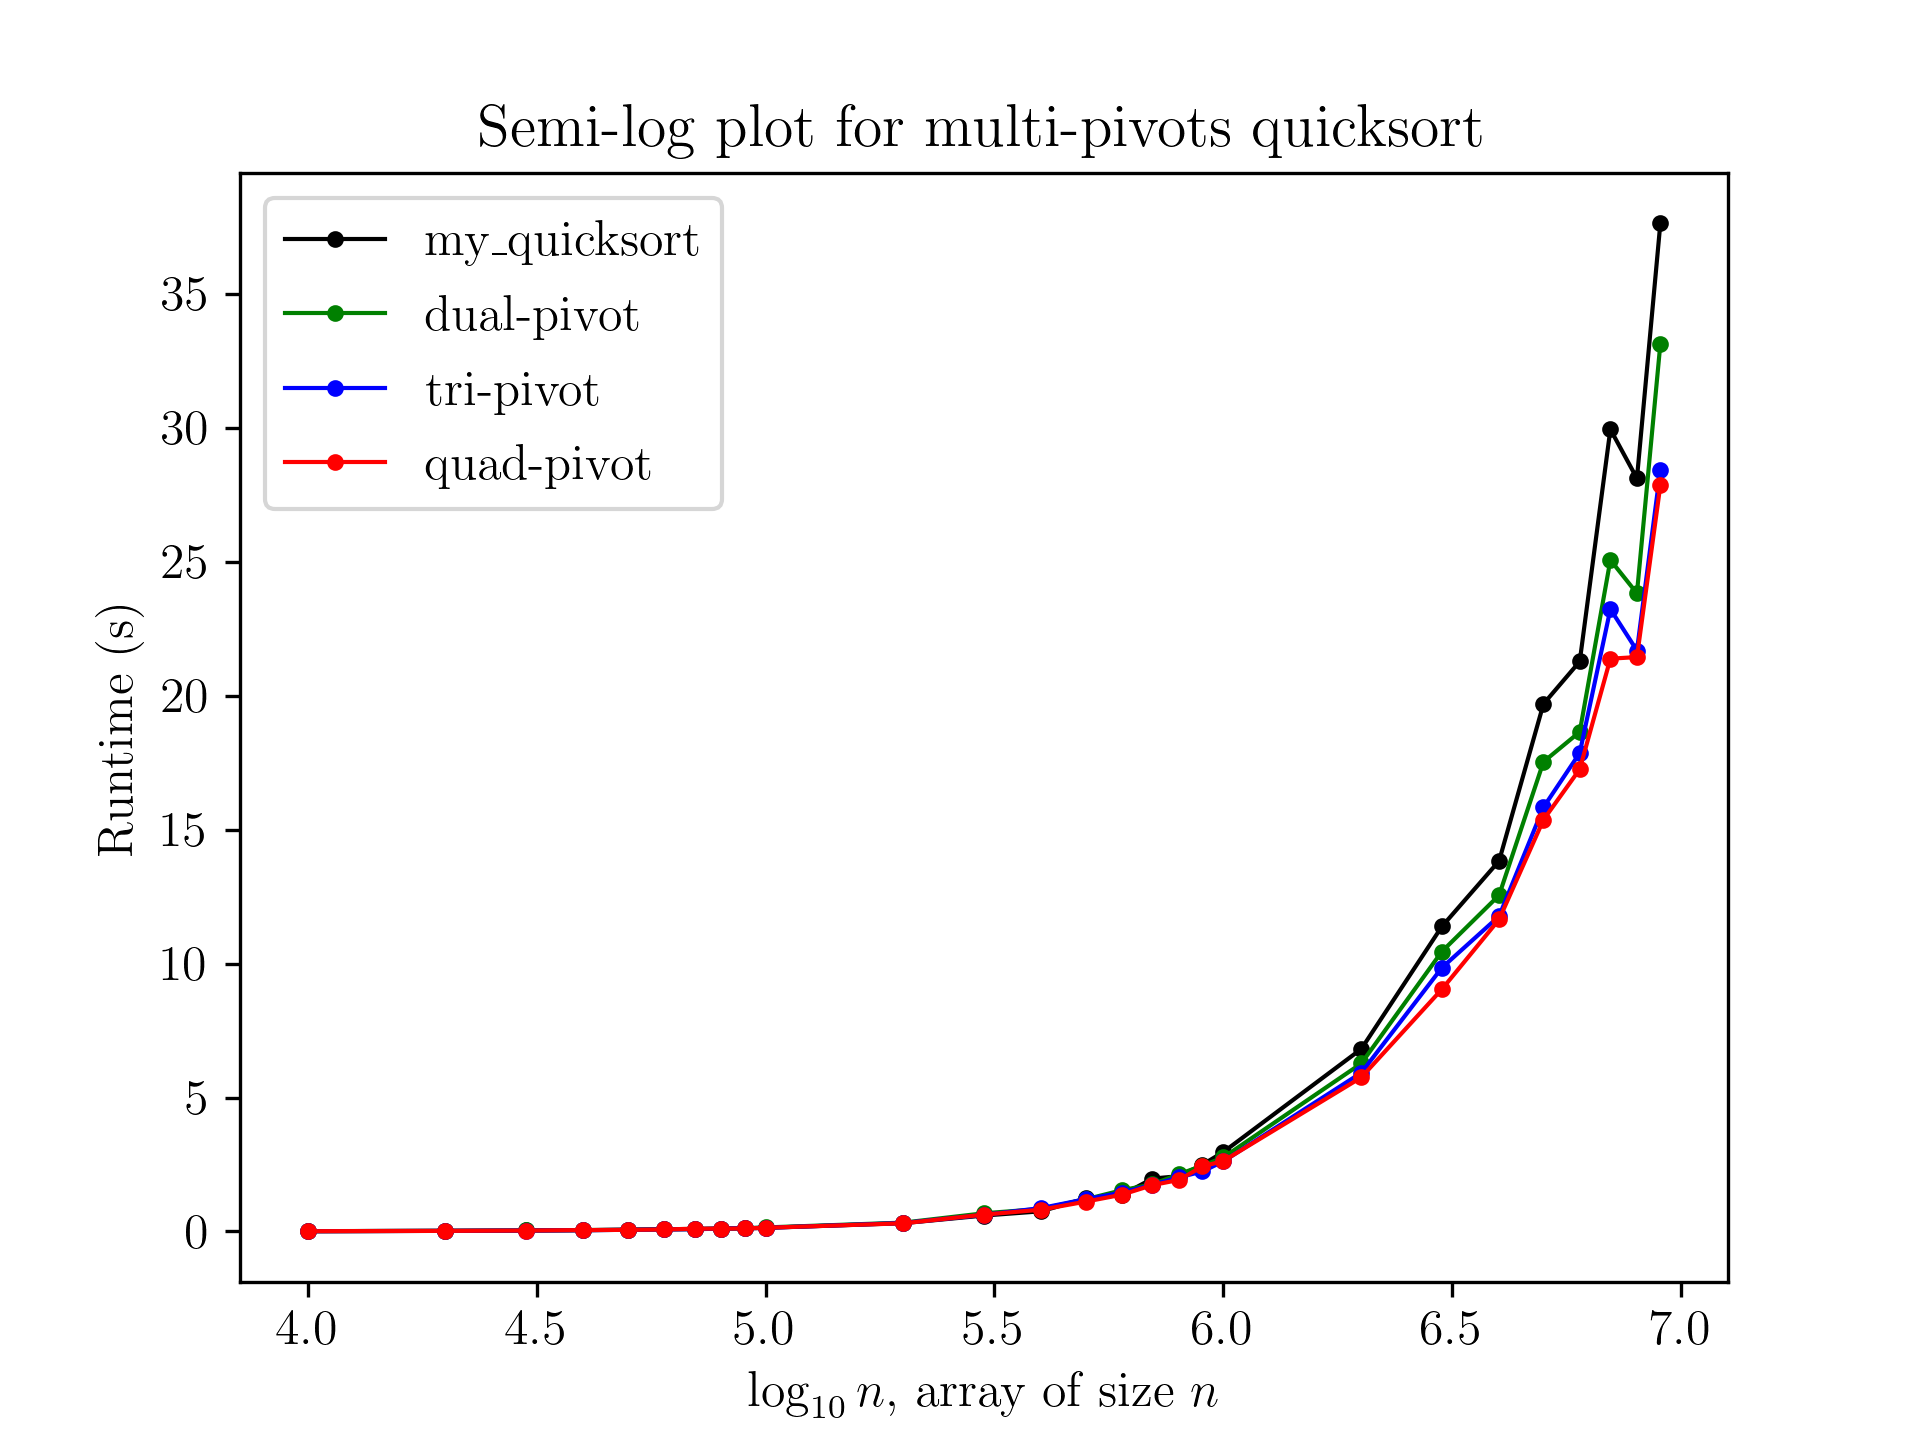
\includegraphics[width=0.8\textwidth]{multp} 
  \caption{Multi-pivot quicksorts runtimes}
  \label{fig:multp}
\end{figure}
\begin{figure}[h]
  \centering
  \begin{subfigure}{0.5\textwidth}
    \centering
    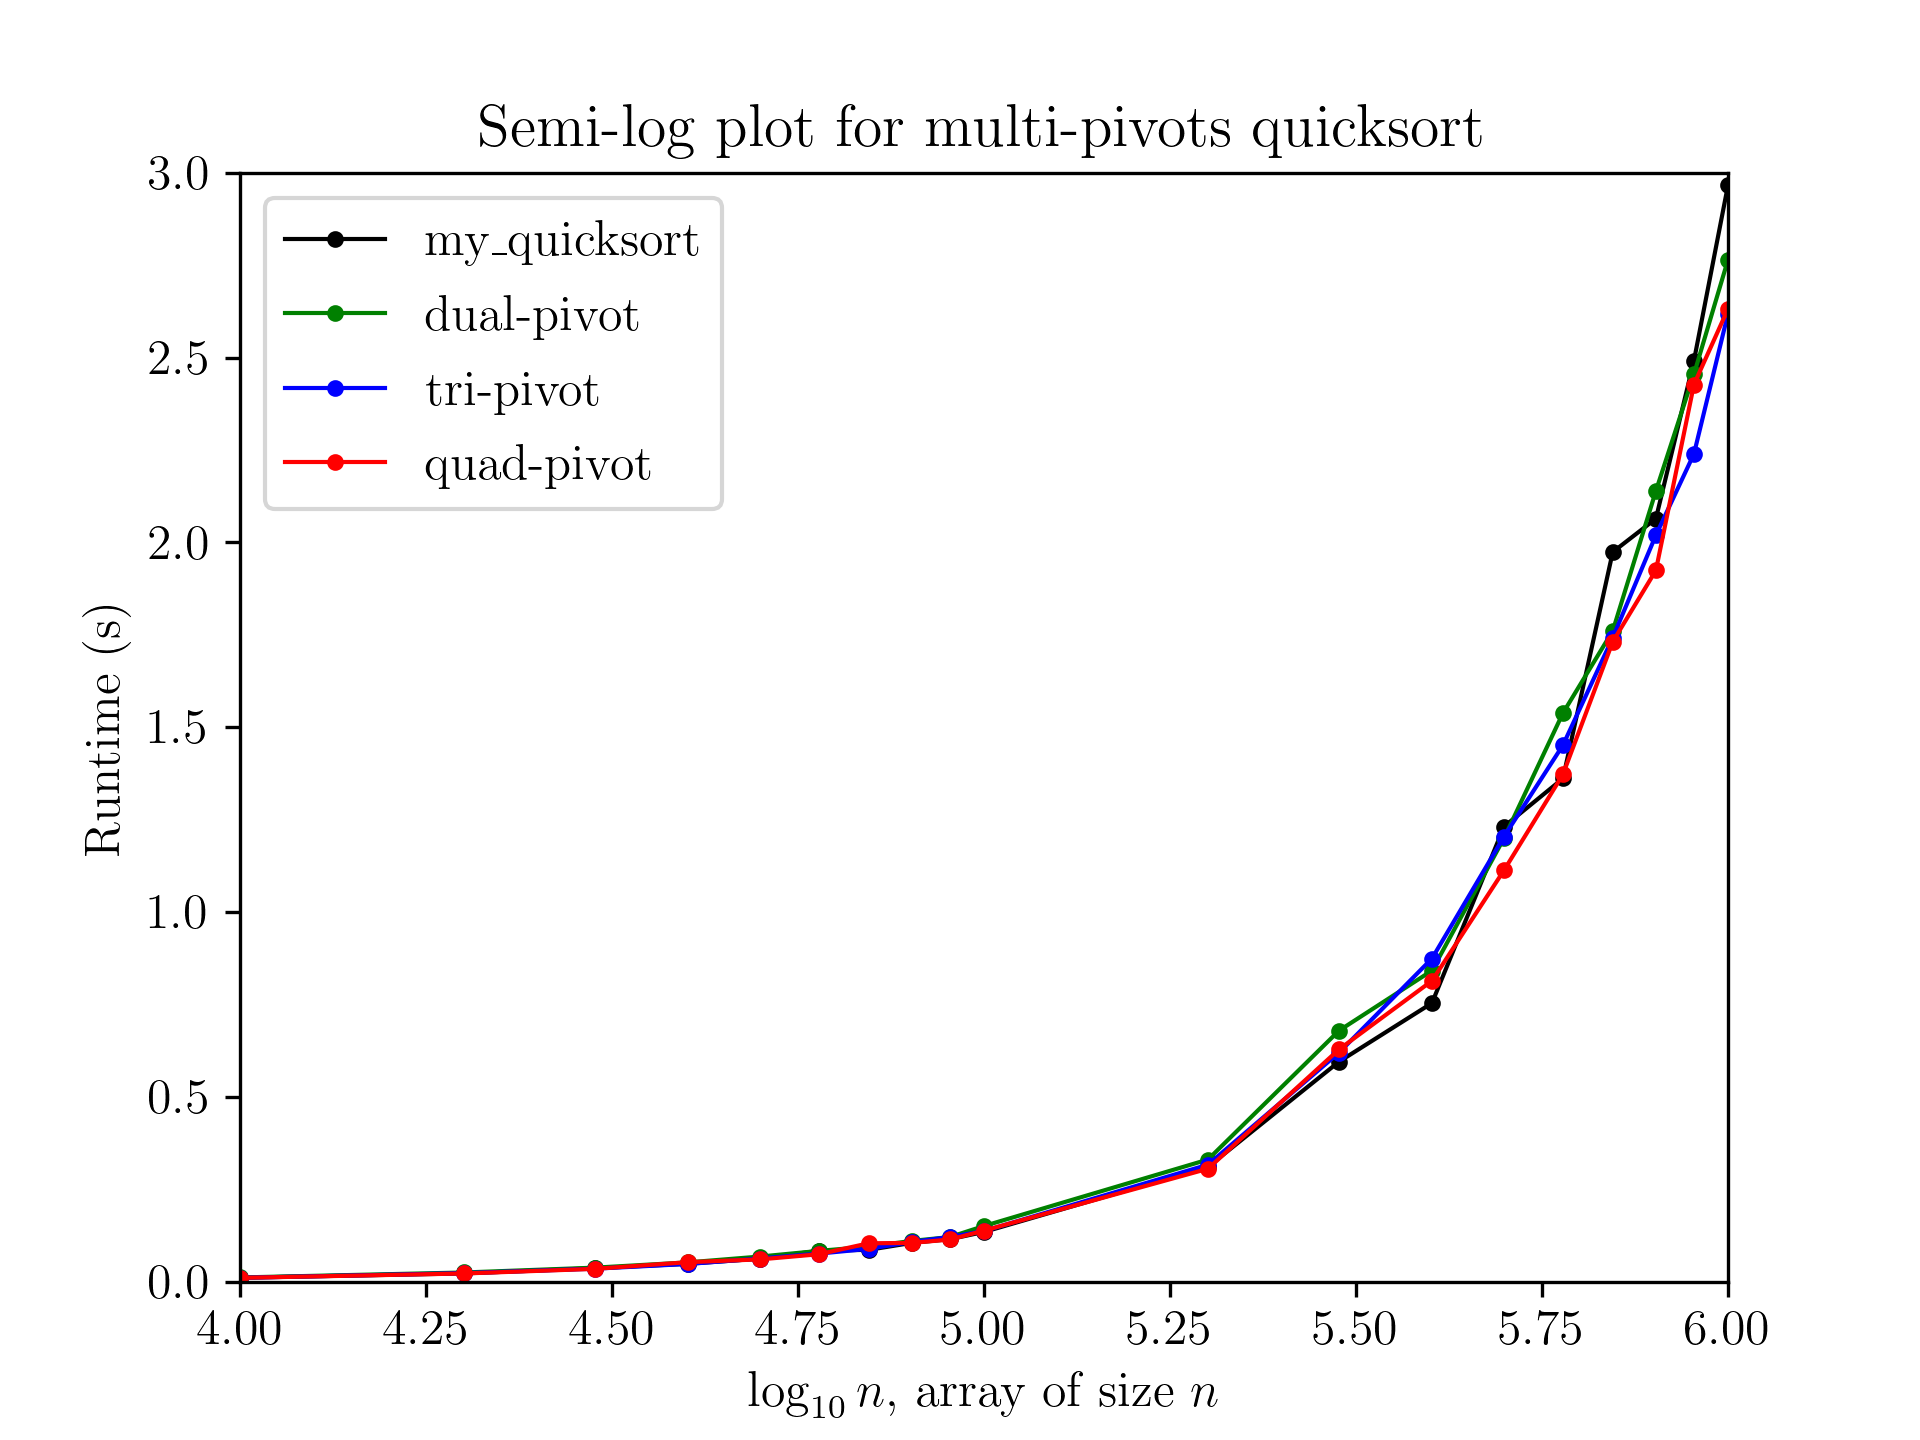
\includegraphics[width=\linewidth]{multp-zoomed-1} 
  \end{subfigure}%
  \begin{subfigure}{0.5\textwidth}
    \centering
    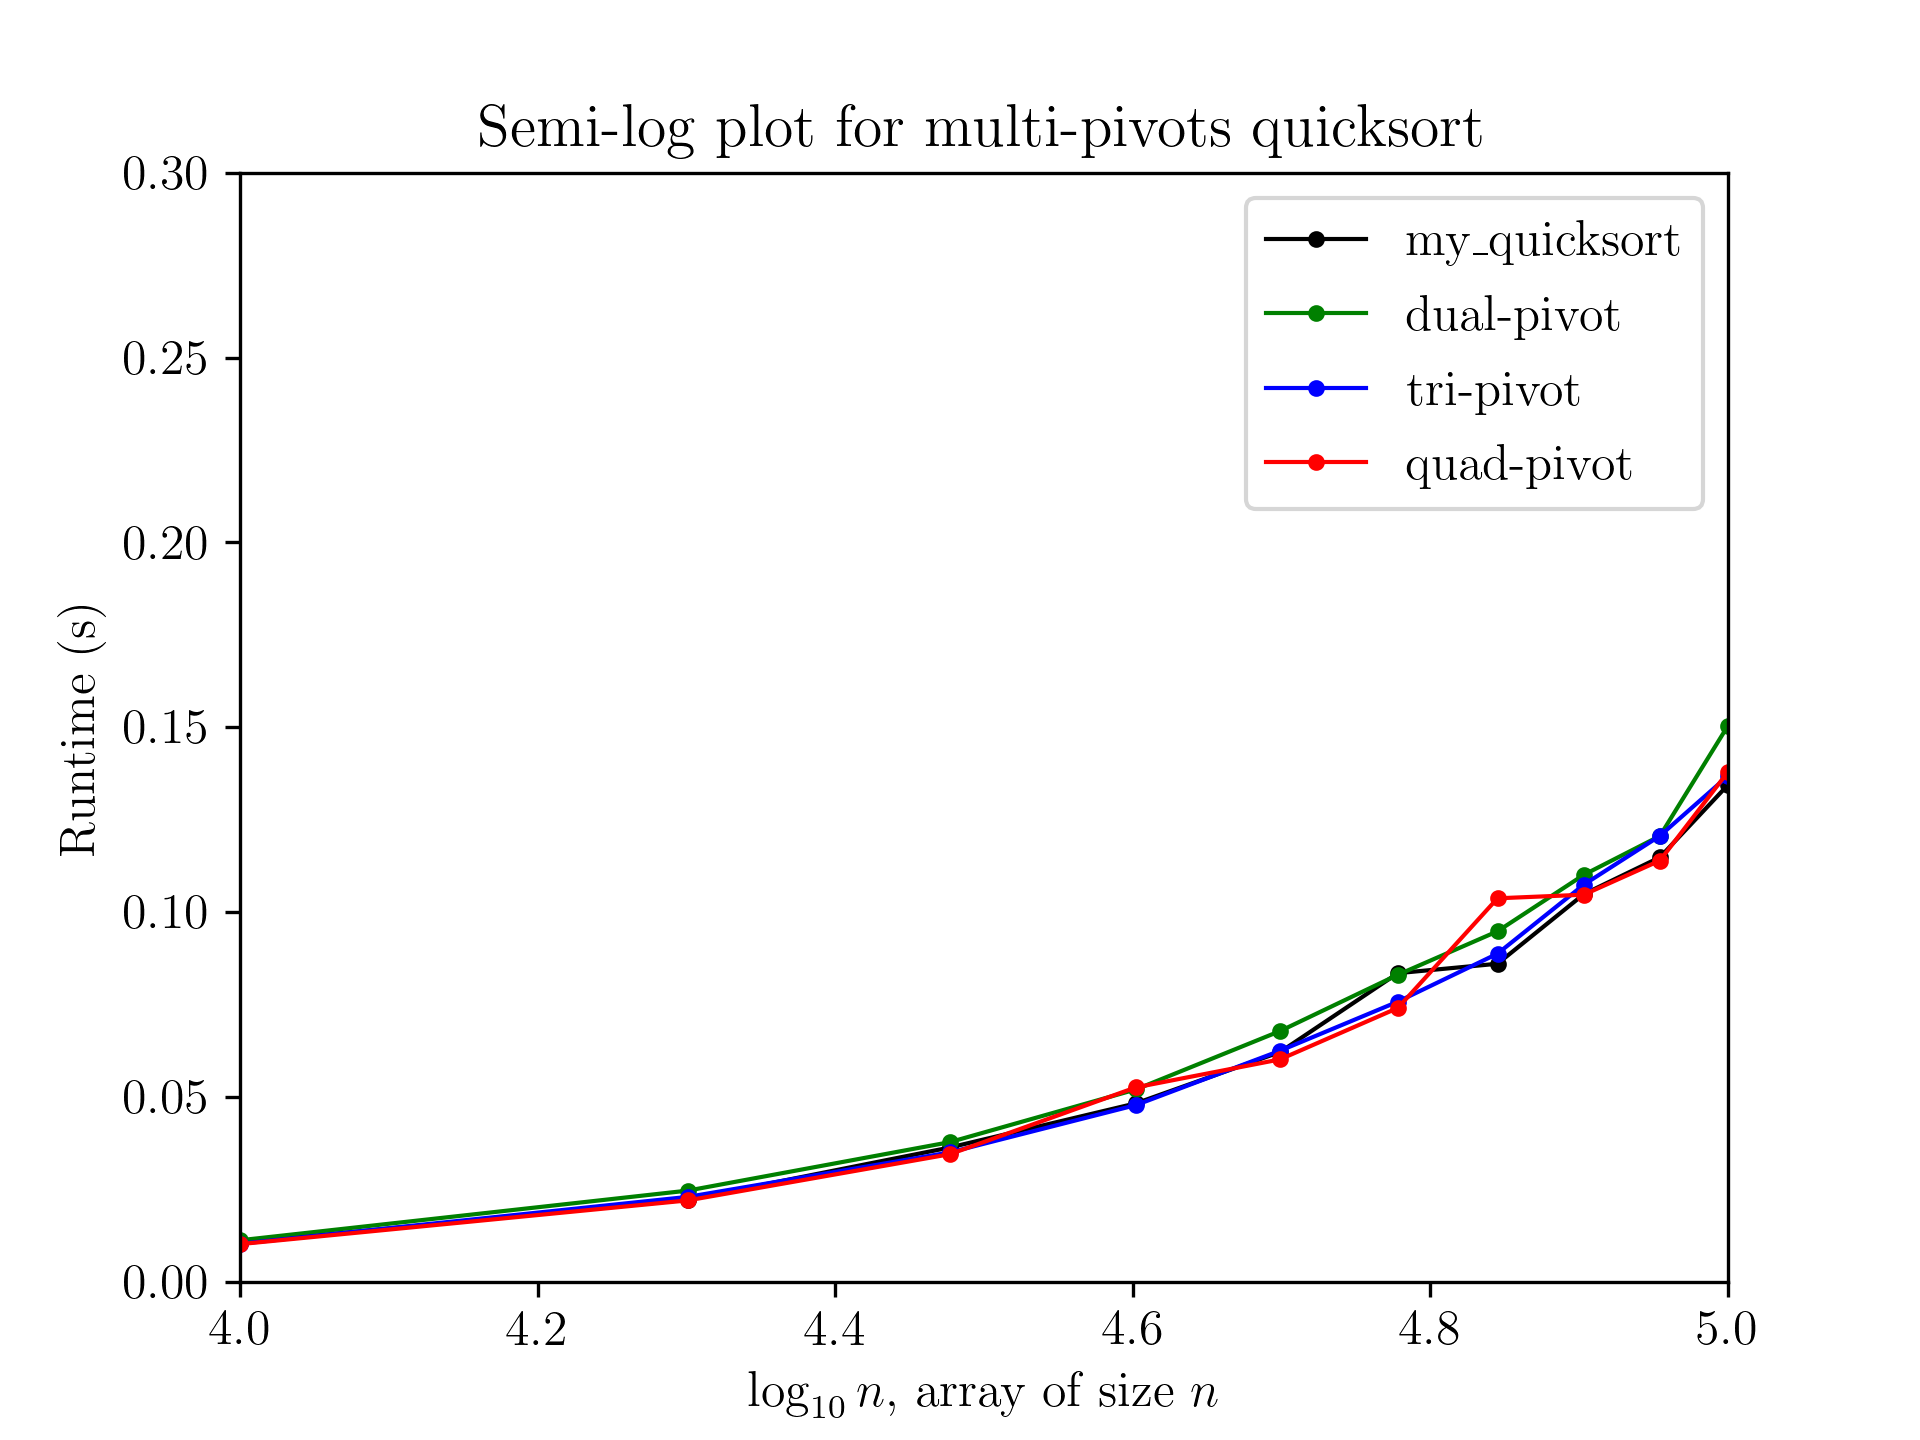
\includegraphics[width=\linewidth]{multp-zoomed-2} 
  \end{subfigure}
  \caption{Quicksort variants on lower scale \( n \)}
  \label{fig:multp-zoomed}
\end{figure}

\subsection{Worstcase Performance}
\label{sec:worst}

The worstcase performance of quicksort happens when the input list is already
sorted in either ascending or descending order and the implementation always
chooses the first or the last element as the pivot. In this case, the algorithm
would only be able to split the list down to two extremely unbalanced
partitions, one with zero length and the other with length \( n - 1 \),
resulting in a \( \sim n \) recursion depth. Also, in each recursion call, \(
\sim n \) comparisons are required to complete the partitioning step. The
overall worst case performance is expected to be \( \mathcal{O}(n^2) \). The
timing experiment result shown in Figure \ref{fig:worst} demonstrates the
significant difference between quicksort on average case and worstcase.

\begin{figure}[h]
  \centering
  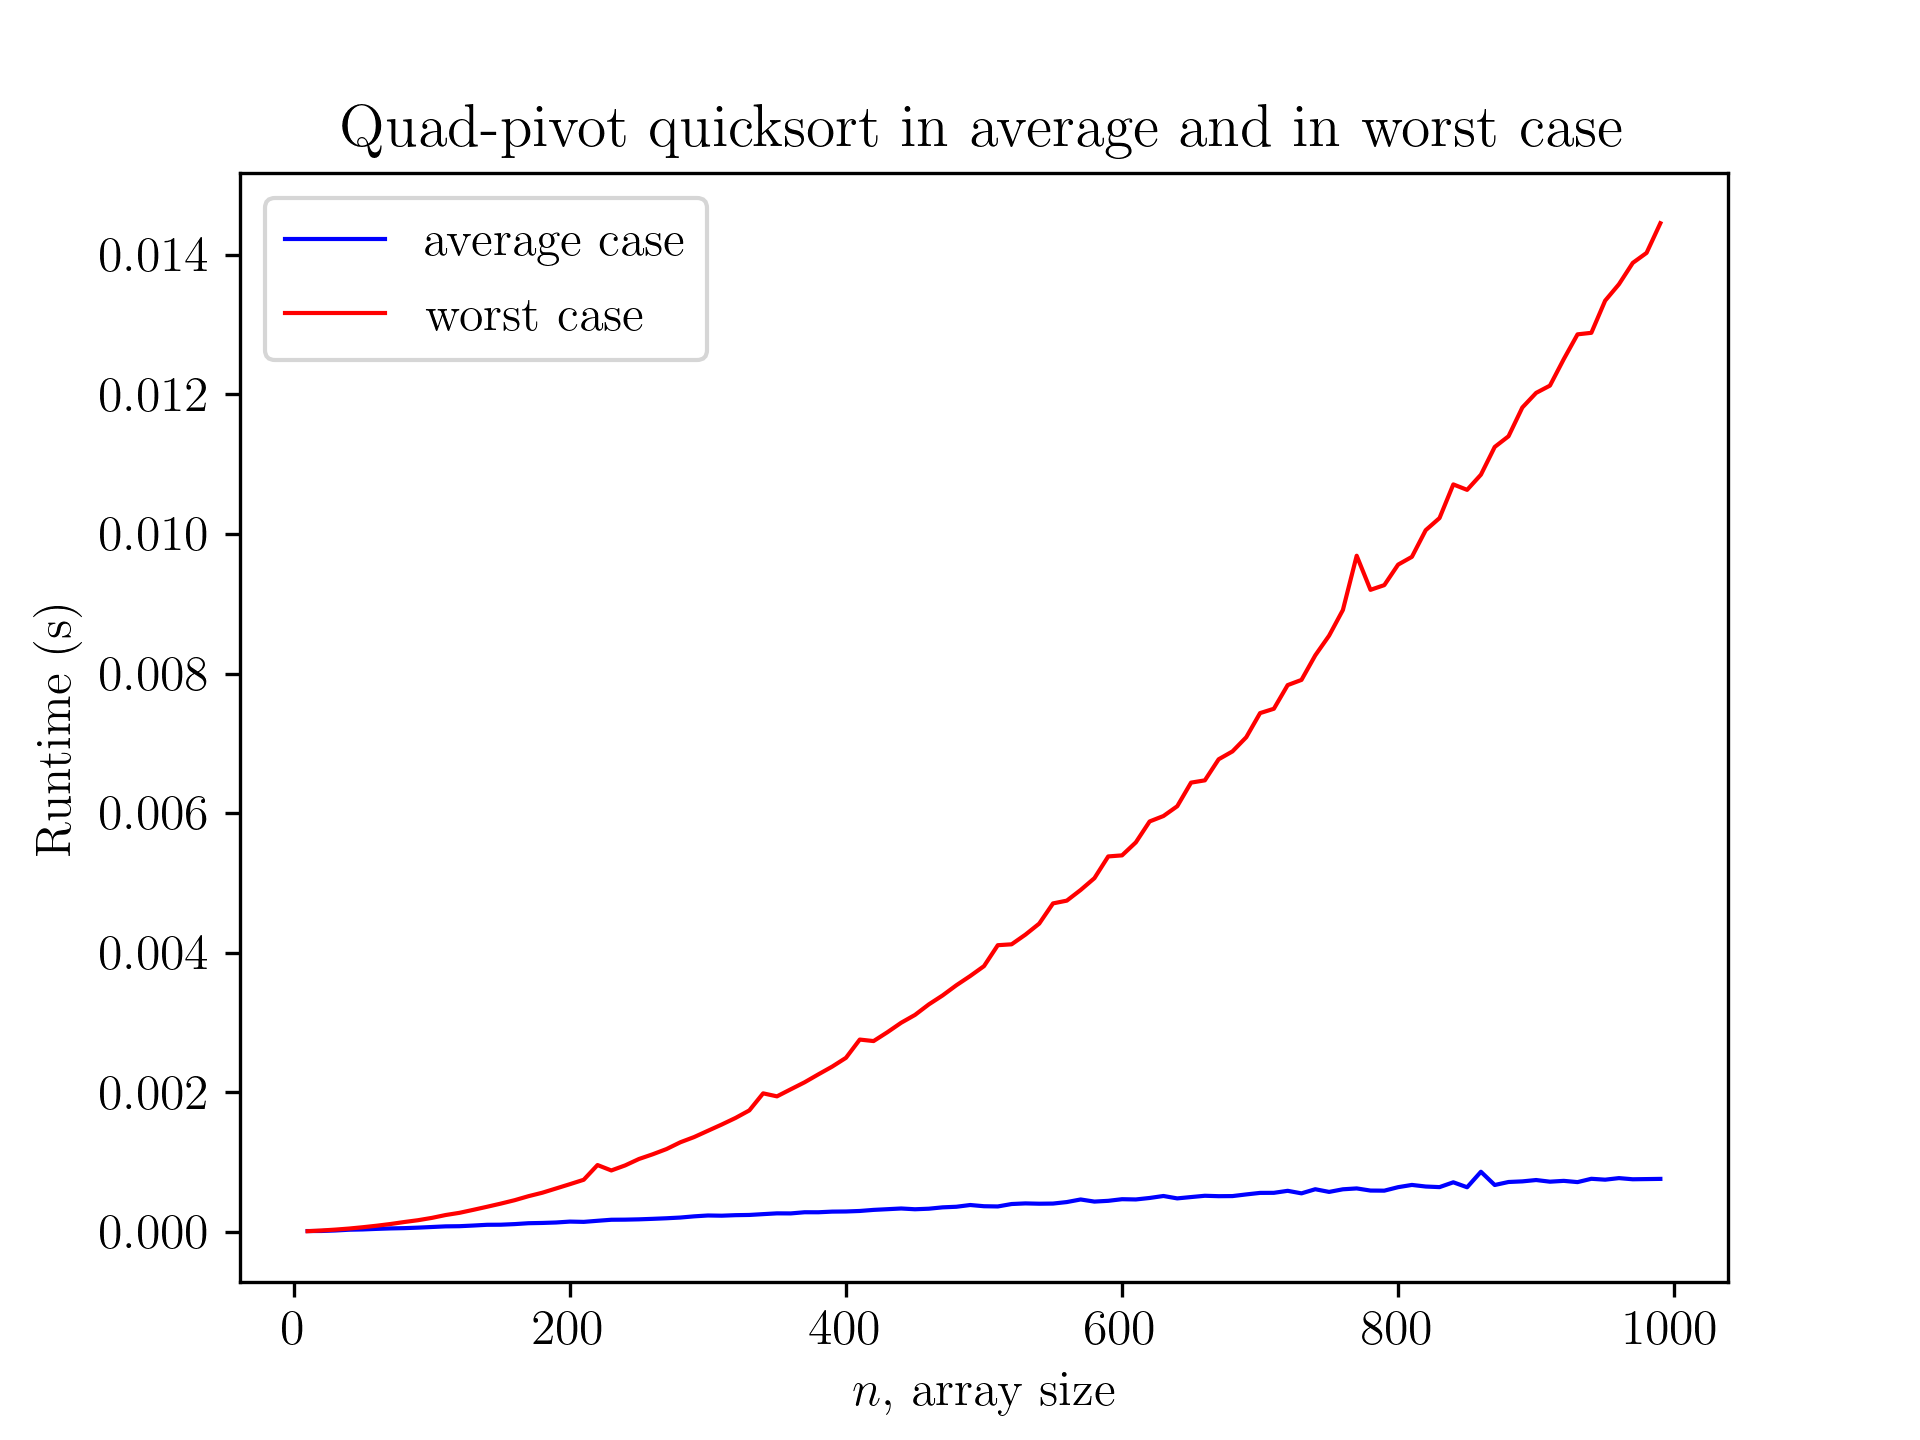
\includegraphics[width=0.8\textwidth]{worst} 
  \caption{Quicksort on average case and worstcase}
  \label{fig:worst}
\end{figure}

For near-sorted lists of elements, insertion sort is expected to outperform
quicksort. This is because quicksort has extra overhead from the recursive
calls, while the core of the insertion sort is simply a \texttt{for} loop.
Focusing on lists of length \( 1000 \), an experiment was conducted to compare
the runtime of four types of sorting algorithms by varying the inversion factor
of an input list. The inversion factor is a percentage of how many elements in a
list are inverted in order. As discussed previously, a sorted (zero inversion)
list is the worstcase for quicksort. Figure \ref{fig:near-sorted} reflects the
relatively slow runtime of quicksort for lower inversion factors. However,
quicksort took the lead at around 5\% inversion factor and performed
significantly better than other elementary sorting algorithms for higher
inversion factors.

\begin{figure}[h]
  \centering
  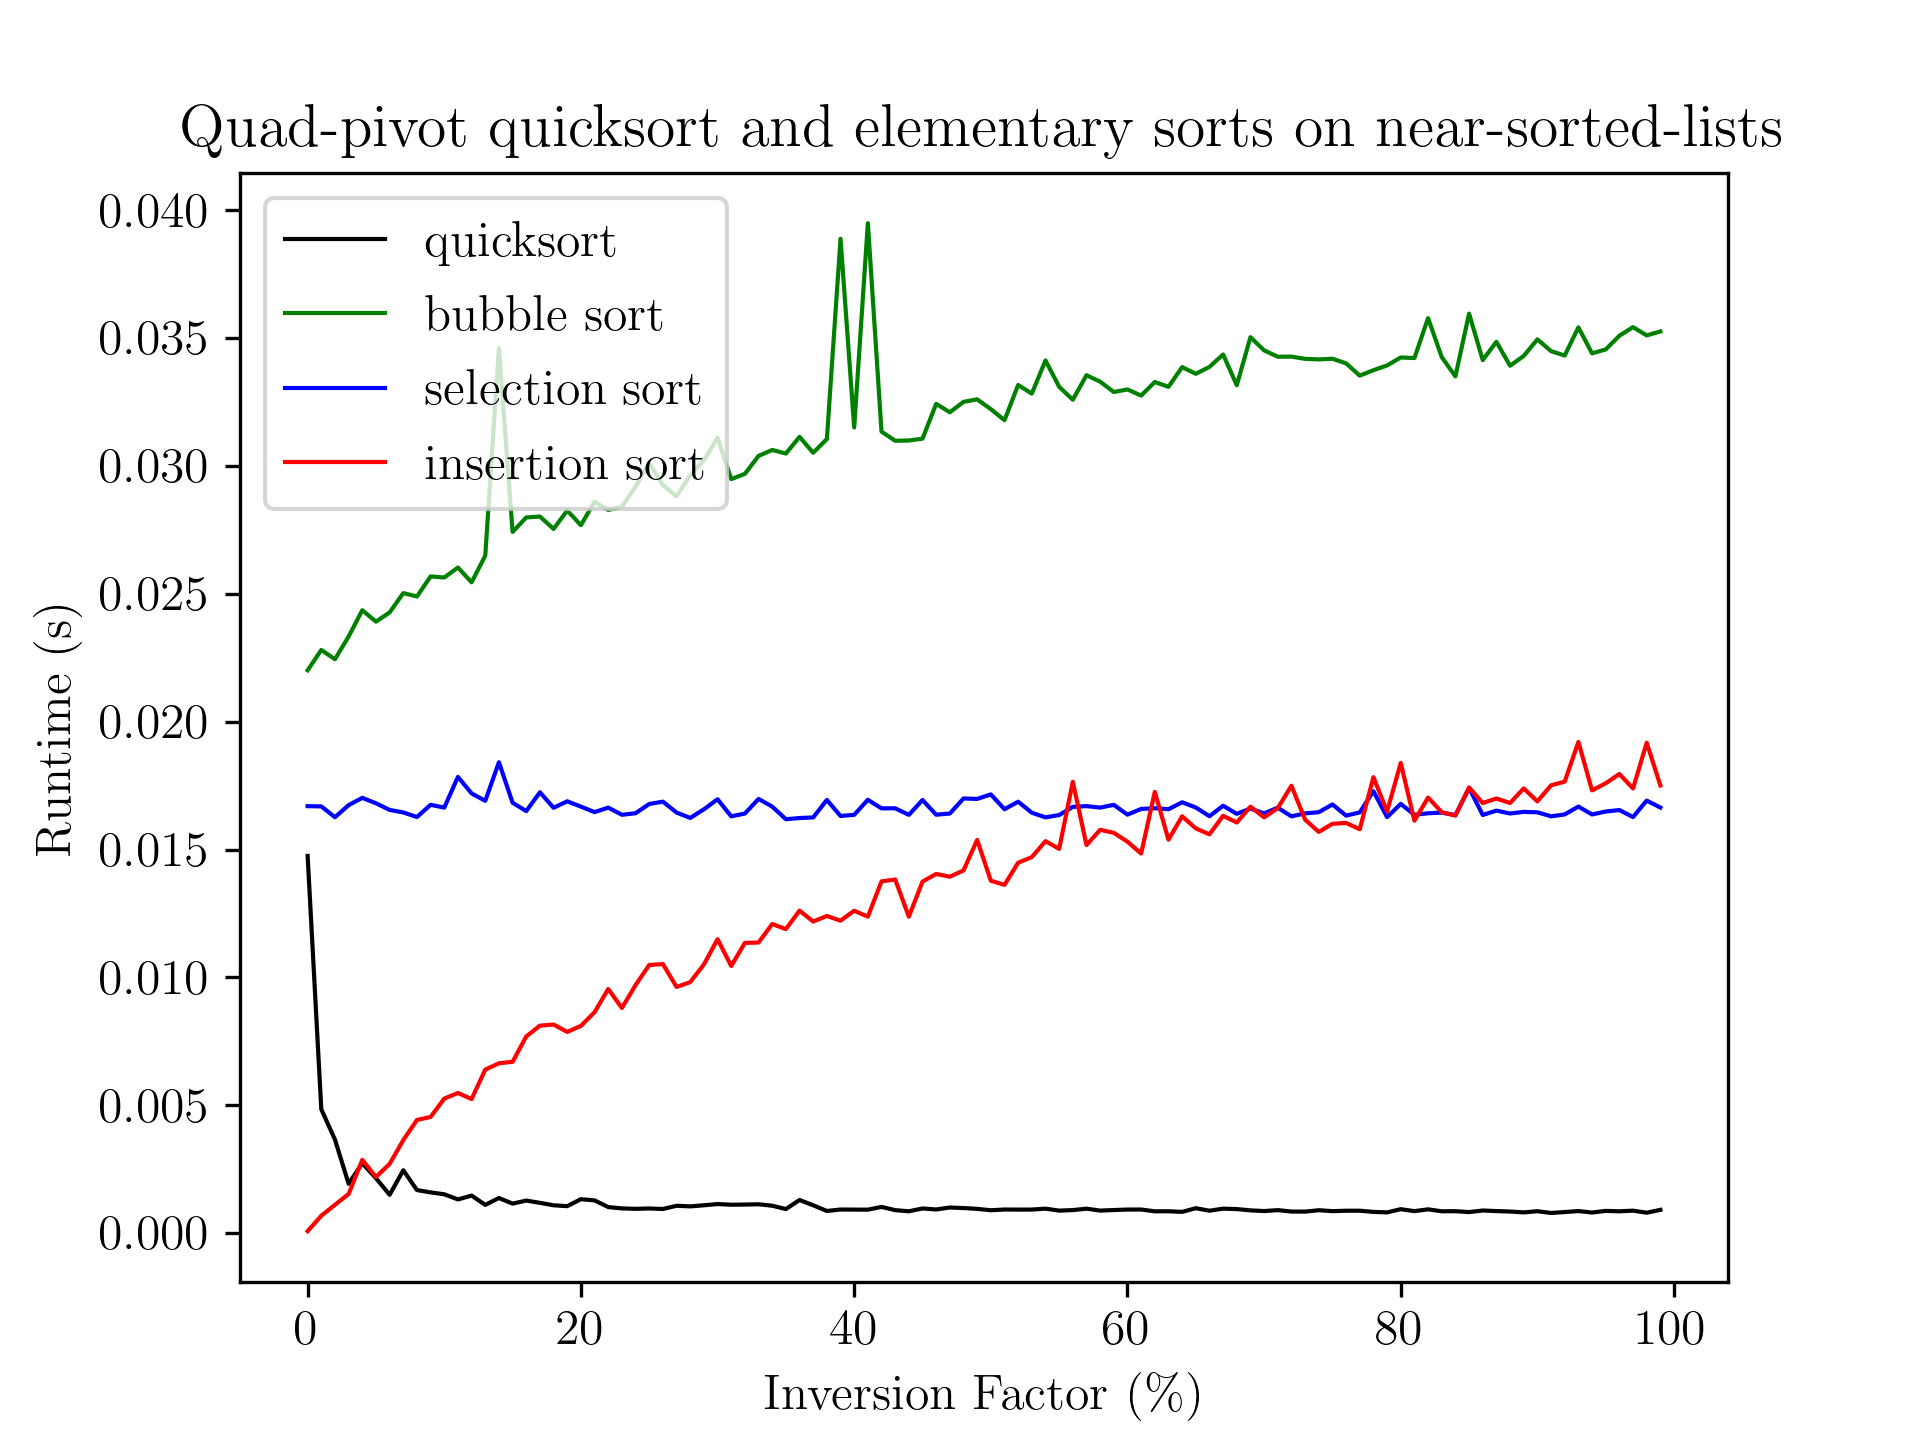
\includegraphics[width=0.8\textwidth]{near-sorted} 
  \caption{Runtime of different sorting algorithms on near-sorted-lists}
  \label{fig:near-sorted}
\end{figure}

\subsection{Small Lists}
\label{sec:small}

The experiment focused on small size lists, for input size \( 1 \leq n \leq 20
\), the insertion sort performed the best compared to other three sorting
algorithms as shown in Figure \ref{fig:small}. A small list has fewer unsorted
elements than a large list, which shares some similarity with a near sorted
list. And the insertion sort performed similarly in both two experiments.
Therefore, insertion sort is the optimal approach while handling small size
lists.

\begin{figure}[h]
  \centering
  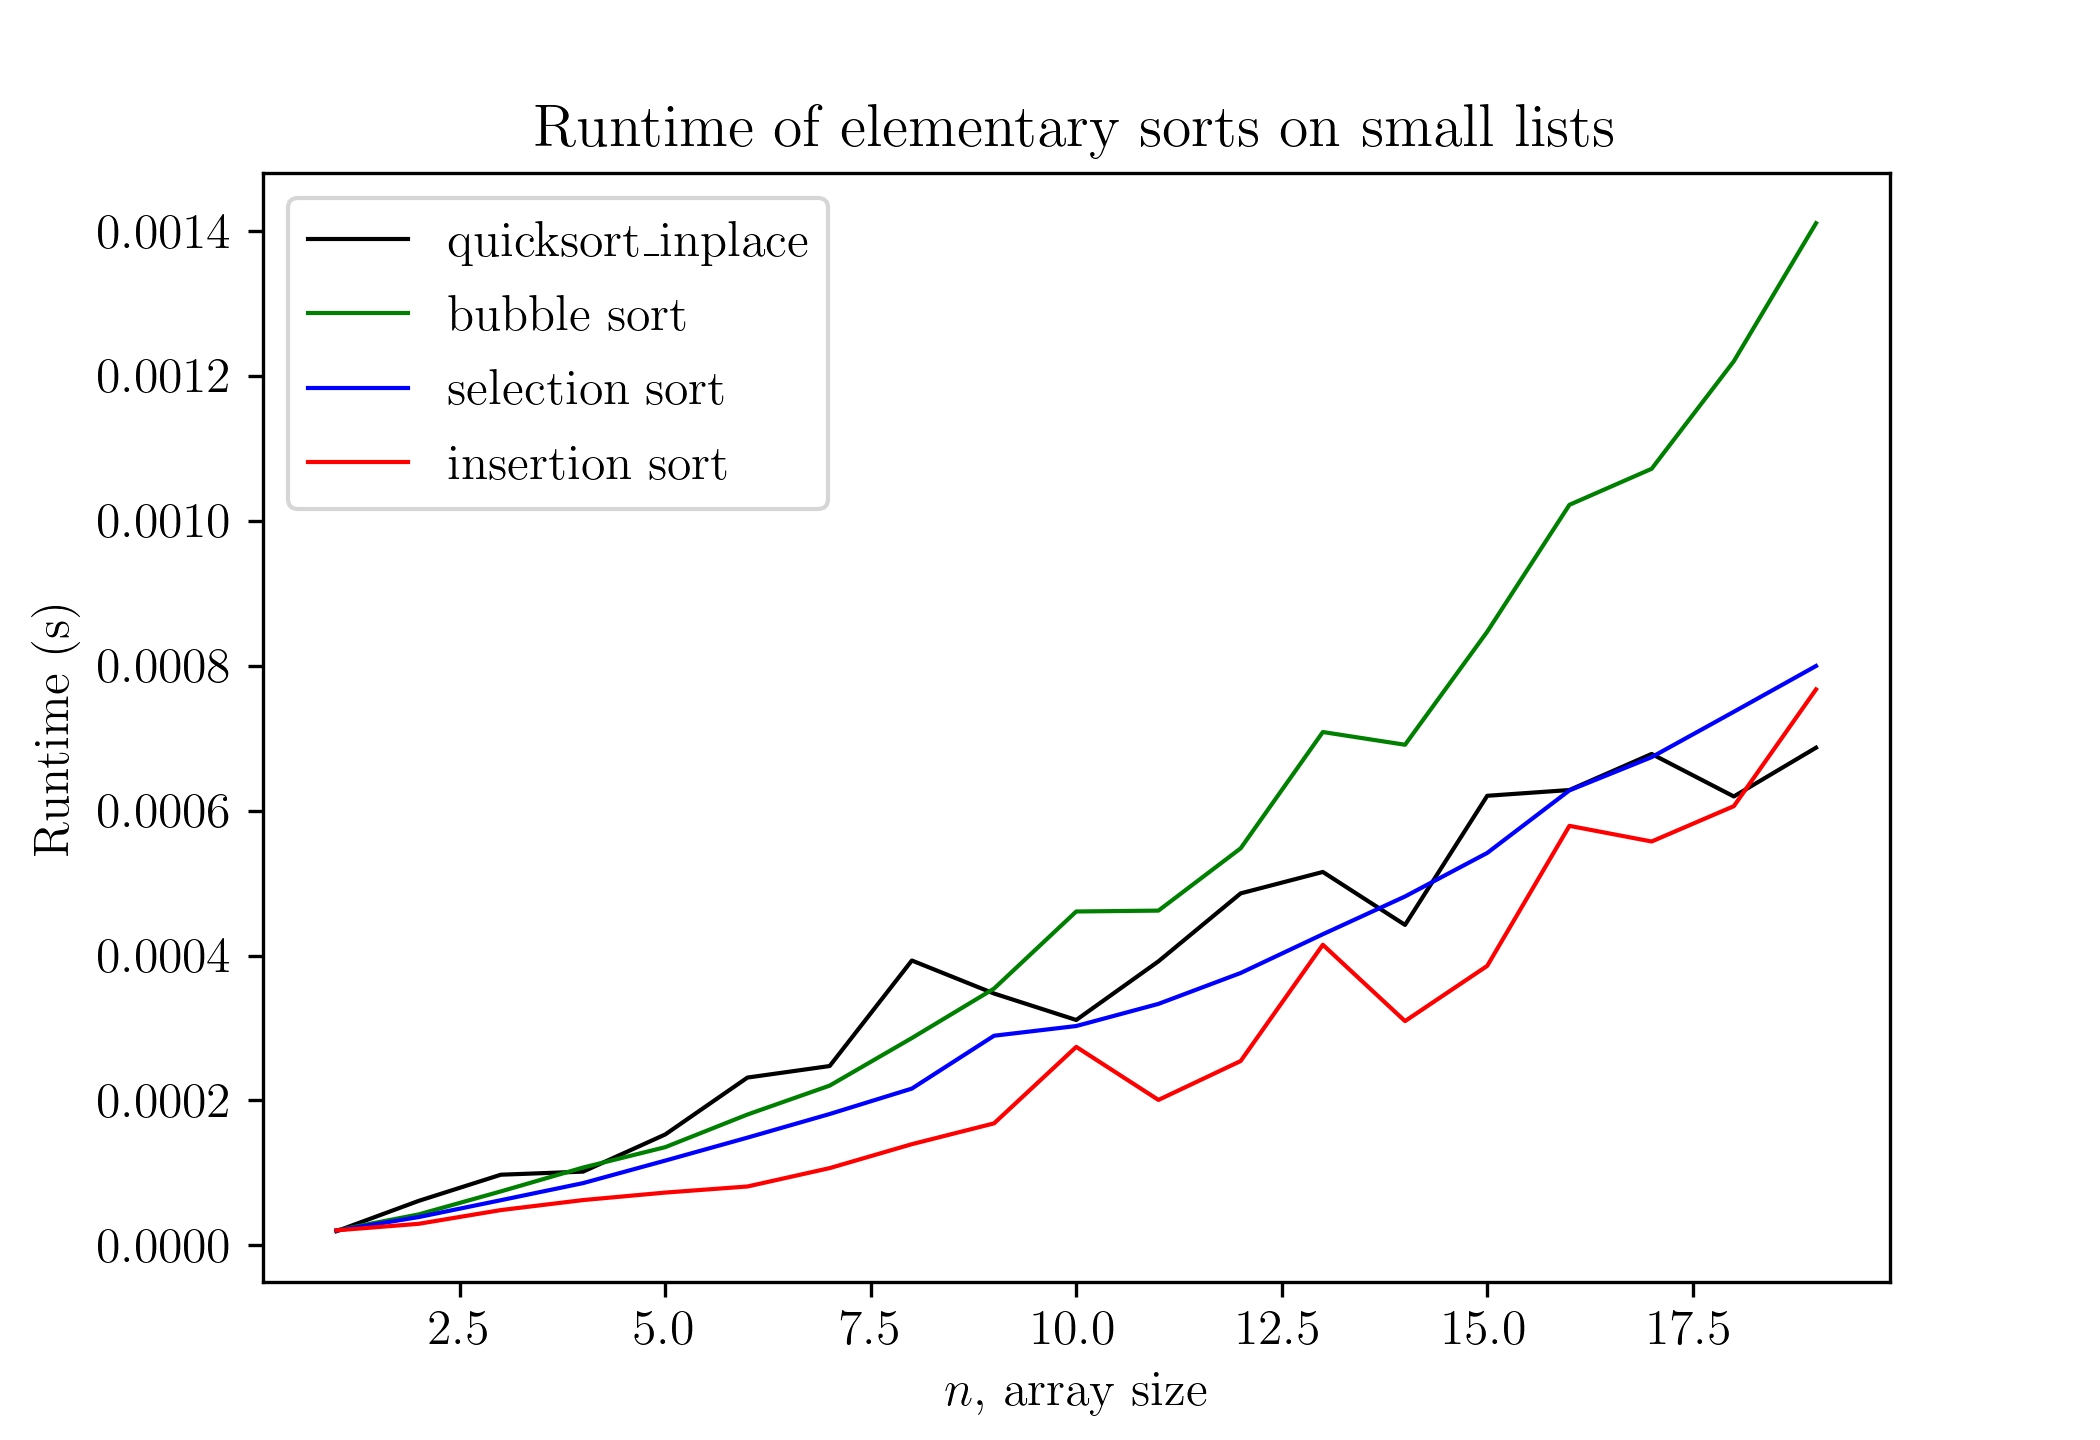
\includegraphics[width=0.8\textwidth]{small}
  \caption{Runtime of different sorting algorithms on small lists}
  \label{fig:small}
\end{figure}

To summarize all the experiments above, we decided to define our
\texttt{final\_sort} to be a hybrid of insertion sort and quad-pivot quicksort.
When the length of the input list is sufficiently short (less than 20), we would
use insertion sort. For any other lists with longer lengths, we would use
quad-pivot quicksort.

The purpose of designing this hybrid algorithm is to minimize the average
runtime. From Section \ref{sec:in-place}, even though the in-place version of
quicksort is faster than the non-in-place version on large scaled lists, it is
still slower than the quad-pivot variant tested in Section \ref{sec:multp}.
Furthermore, from Section \ref{sec:small}, insertion sort has an observable
advantage over other algorithms in terms of runtime for lists of length 20 and
below. As for the lessons learned from Section \ref{sec:worst}, near-sorted
lists in descending order are worstcase for both insertion sort and quicksort
with \( \mathcal{O}(n^2) \) complexity, while ascending ordered lists are best
case for insertion sort but worstcase for quicksort. An ideal
insertion-quicksort hybrid sorting algorithm would use insertion sort's best
case to balance out quicksort's worstcase for ascending sorted lists. However,
there is not sufficiently efficient algorithm to determine whether an input list
is near-sorted. One possible solution to balance the worstcase for quicksort is
to use a randomized quicksort. However, such implementation is beyond the scope
of the lab. Therefore, we conclude that a hybrid sorting algorithm comprises
insertion sort and quicksort which conditionally chooses a sorting algorithm
based on the input size, is the best performing sorting algorithm on average
case.

\end{document}
